%ALLEGATI IN FONDO A TUTTO:
\appendix
%\renewcommand{\thechapter}{Allegati} %Toglie A,B,C delle appendici del TOC sostituendolo con "Allegati"
%Funziona solo perché c'è solo un appendice sennò non avrebbe senso
\titleformat{\chapter}%toglie A, B, C e sposta il nome a sinistra
        {\normalfont\Huge\bfseries}{}{0em}{} 
\chapter[ALLEGATI]{Allegati} %Nell'indice non ha nome []
\begin{enumerate}
    \item Piante edificio
    \item Zonizzazione dello stato zero
    \item WBS stato zero
    \item Computo metrico estimativo struttura perimetrale
    \item Computo metrico estimativo struttura pareti interne e solai intermedi e di copertura
\end{enumerate}
%\clearpage serve perché i ref venivano sbagliati
%\phantomsection serve perchè l'xyperlink non riportata al punto giusto

%Piante edificio:
%I pdf originali sono in A3 a scala 1:50 in realtà. Ora è diventato in 1:100 A4
%\clearpage
%\phantomsection
%\label{piante}
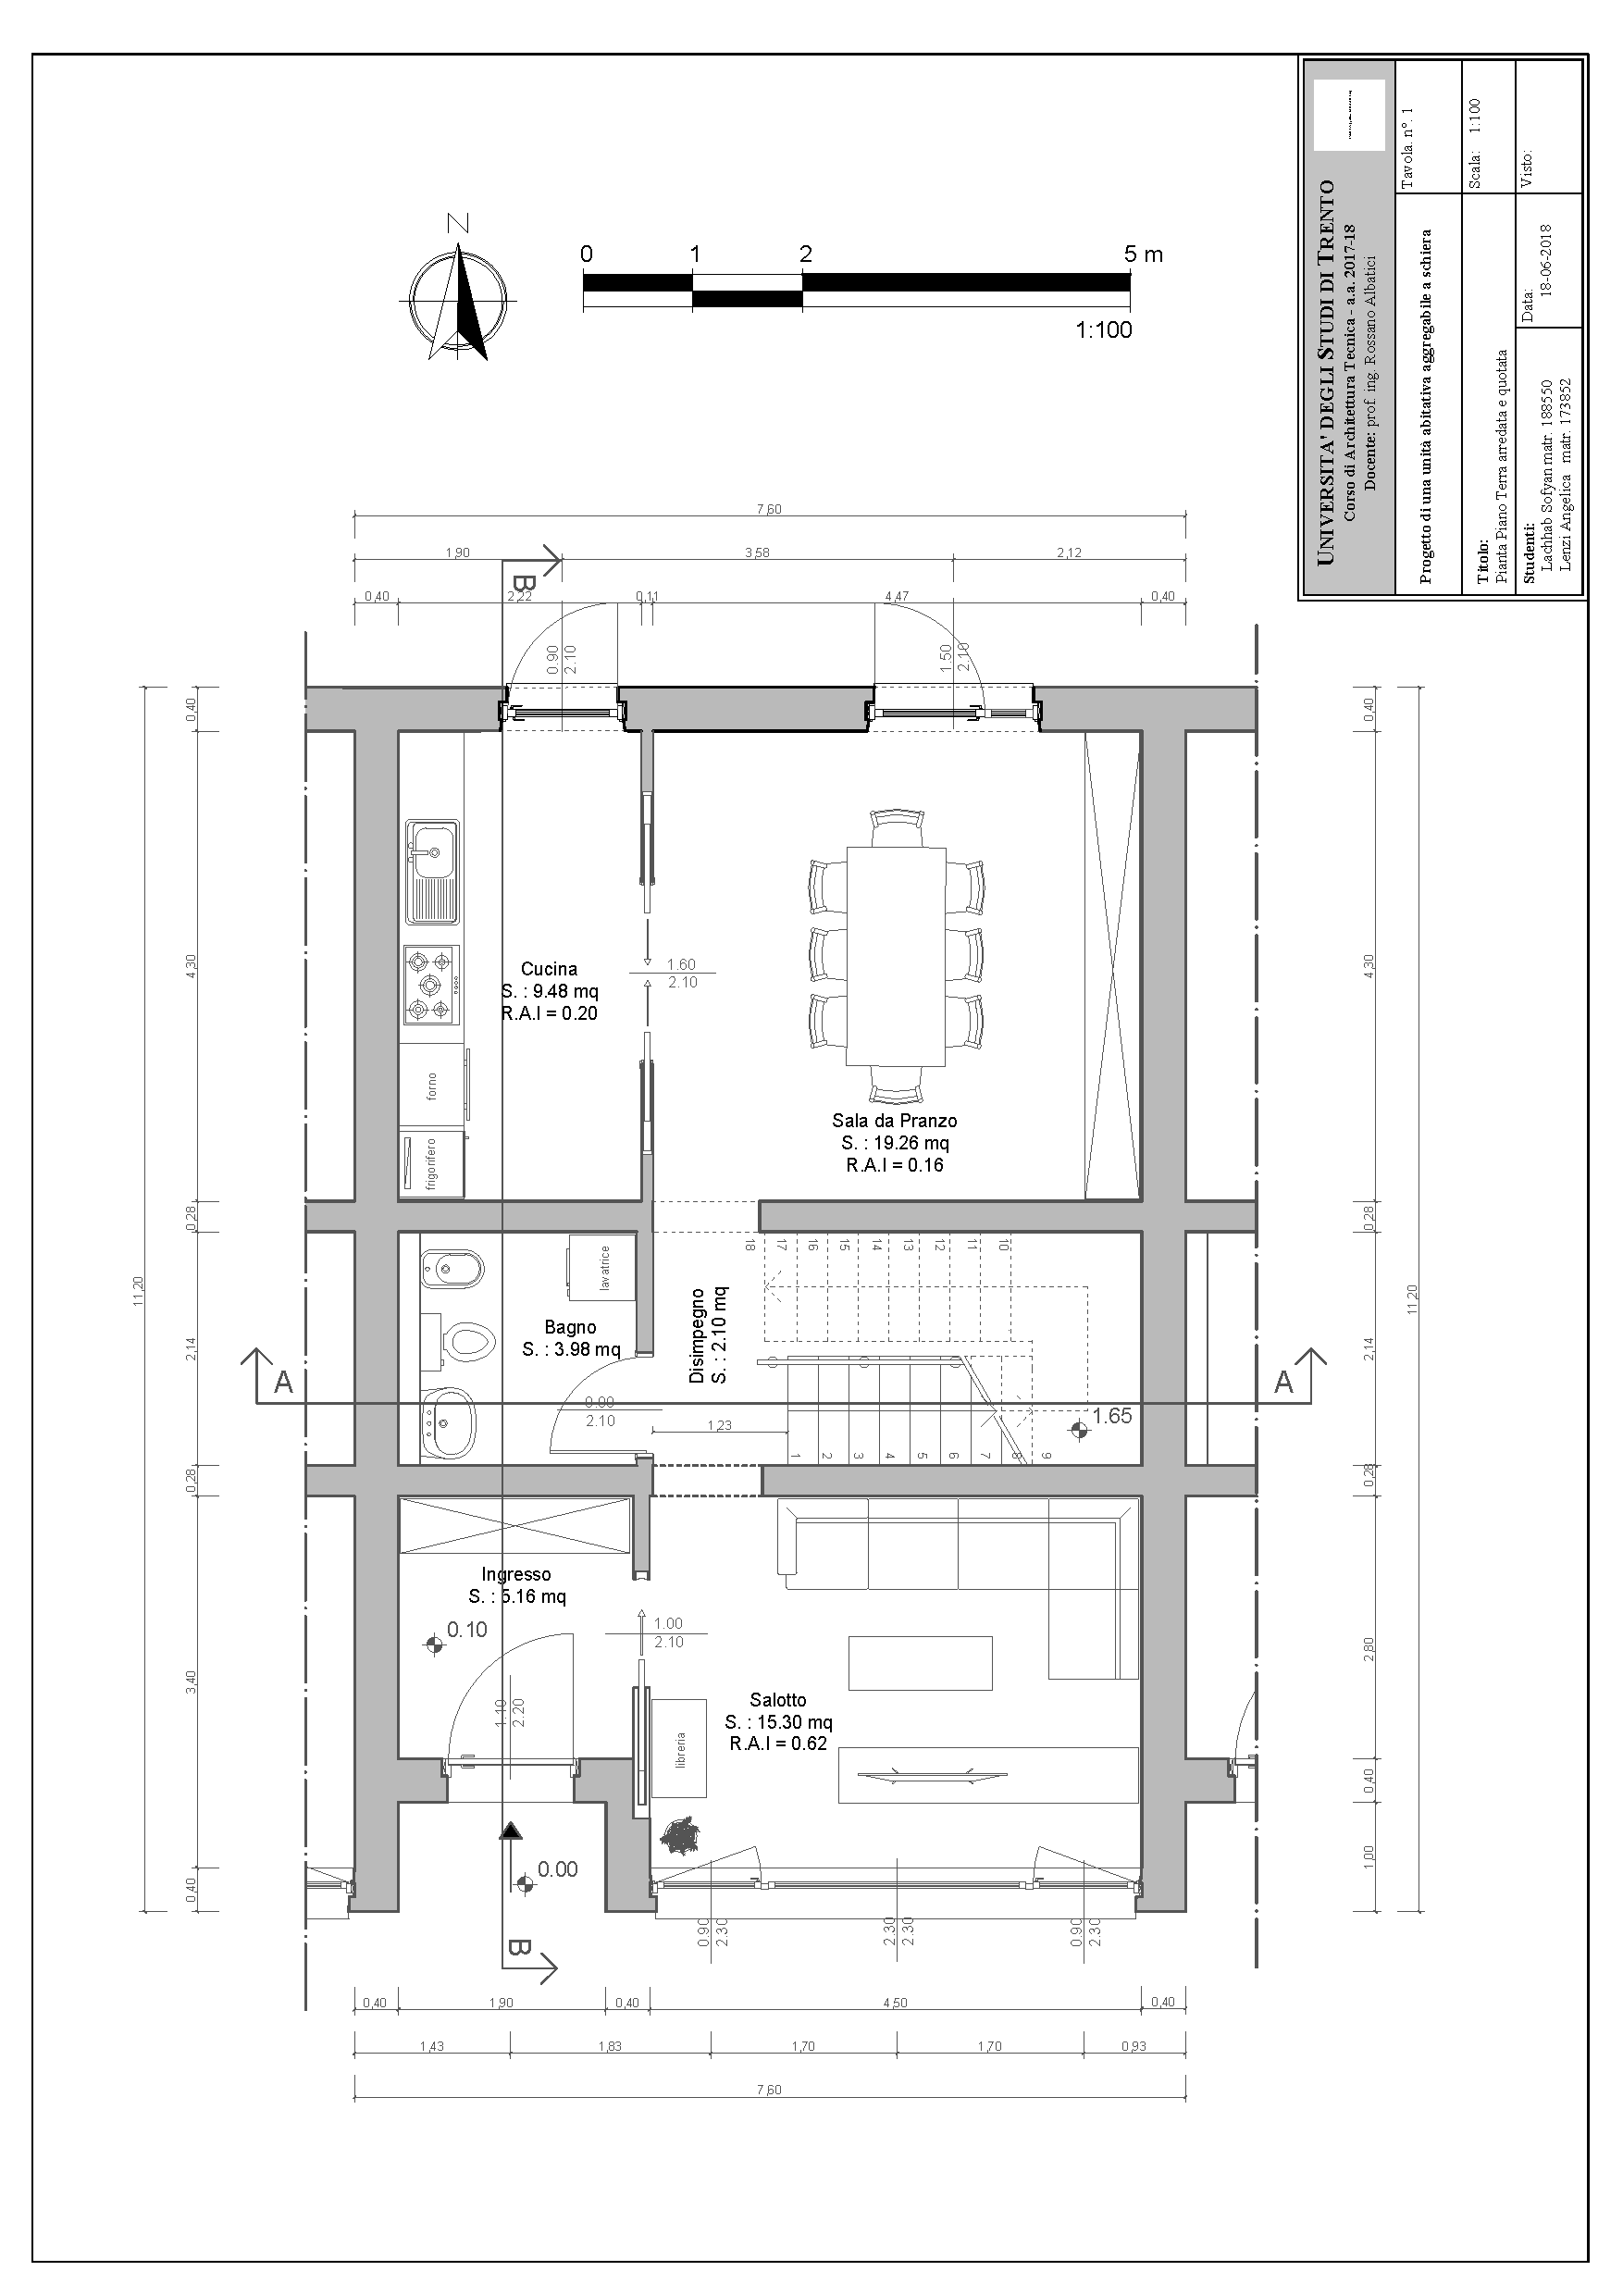
\includepdf[pages={1},pagecommand={\thispagestyle{plain}},addtotoc={1,section,2,Piante edificio,piante}]{img/PiantaTerraA3scala50.pdf}
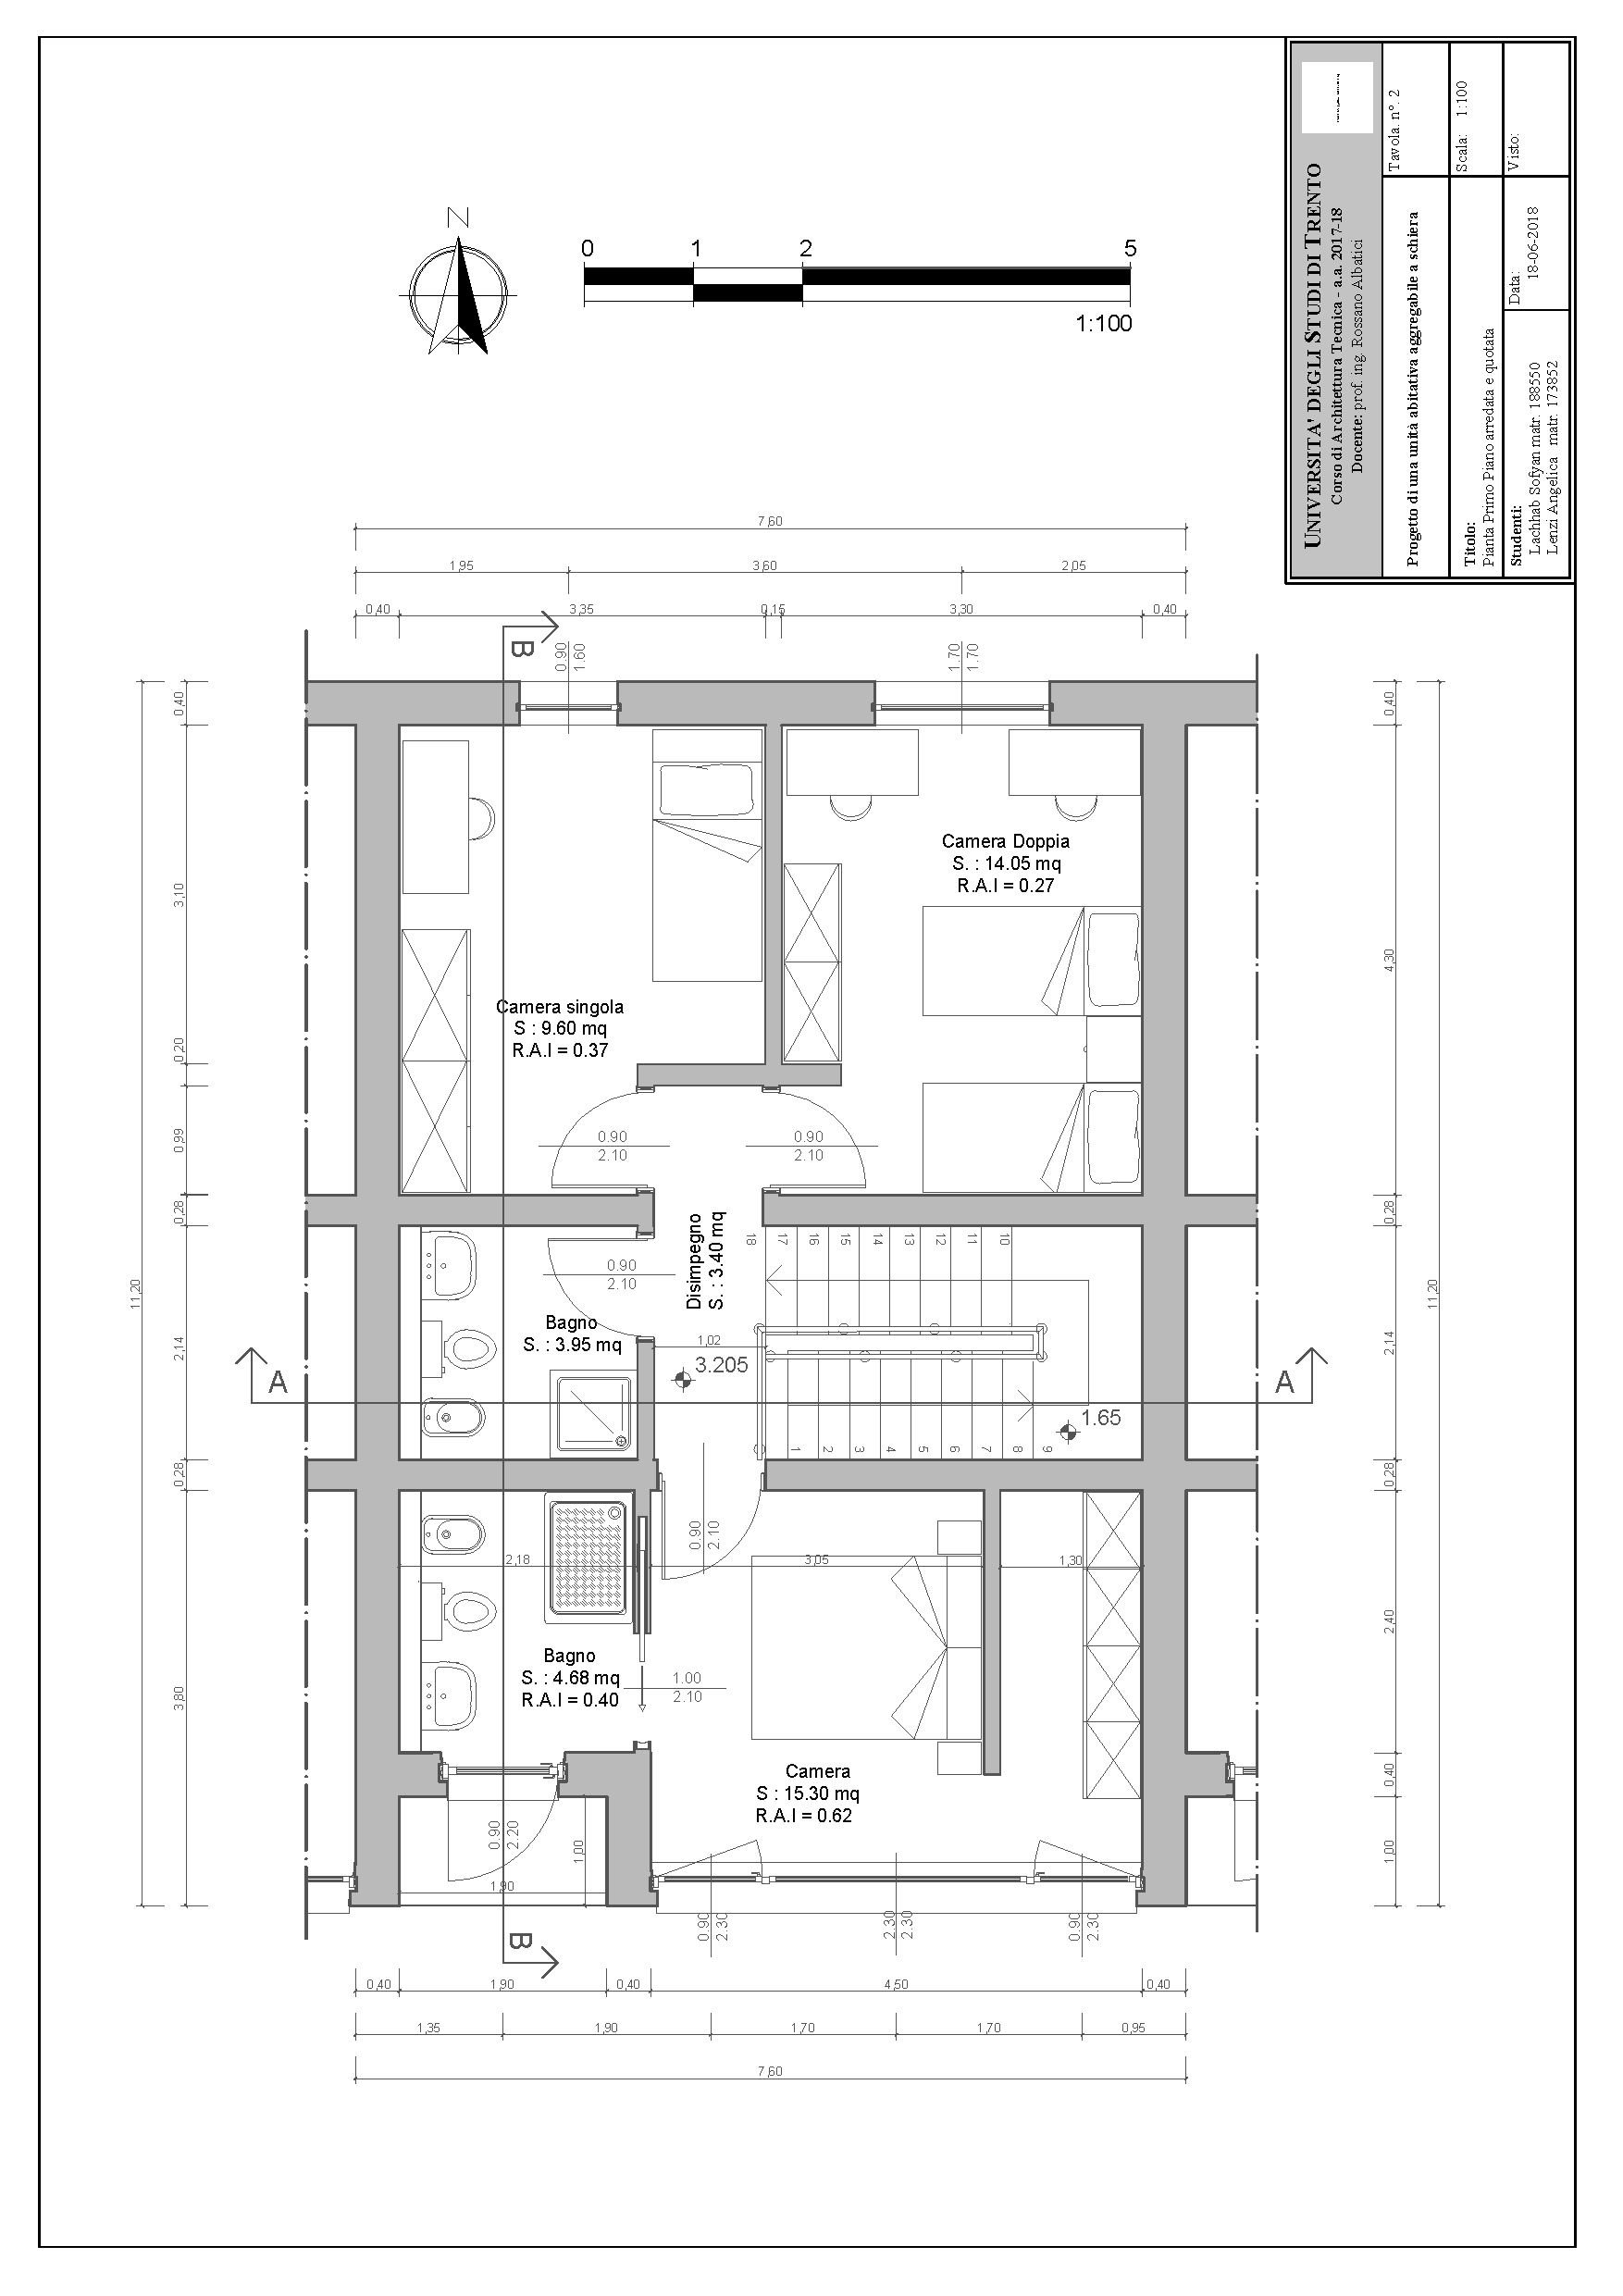
\includepdf[pages={1},pagecommand={\thispagestyle{plain}}]{img/PiantaPrimoA3scala50.pdf}
%Zona ubicazione edificio
%\clearpage
%\phantomsection
%\label{Edificio}
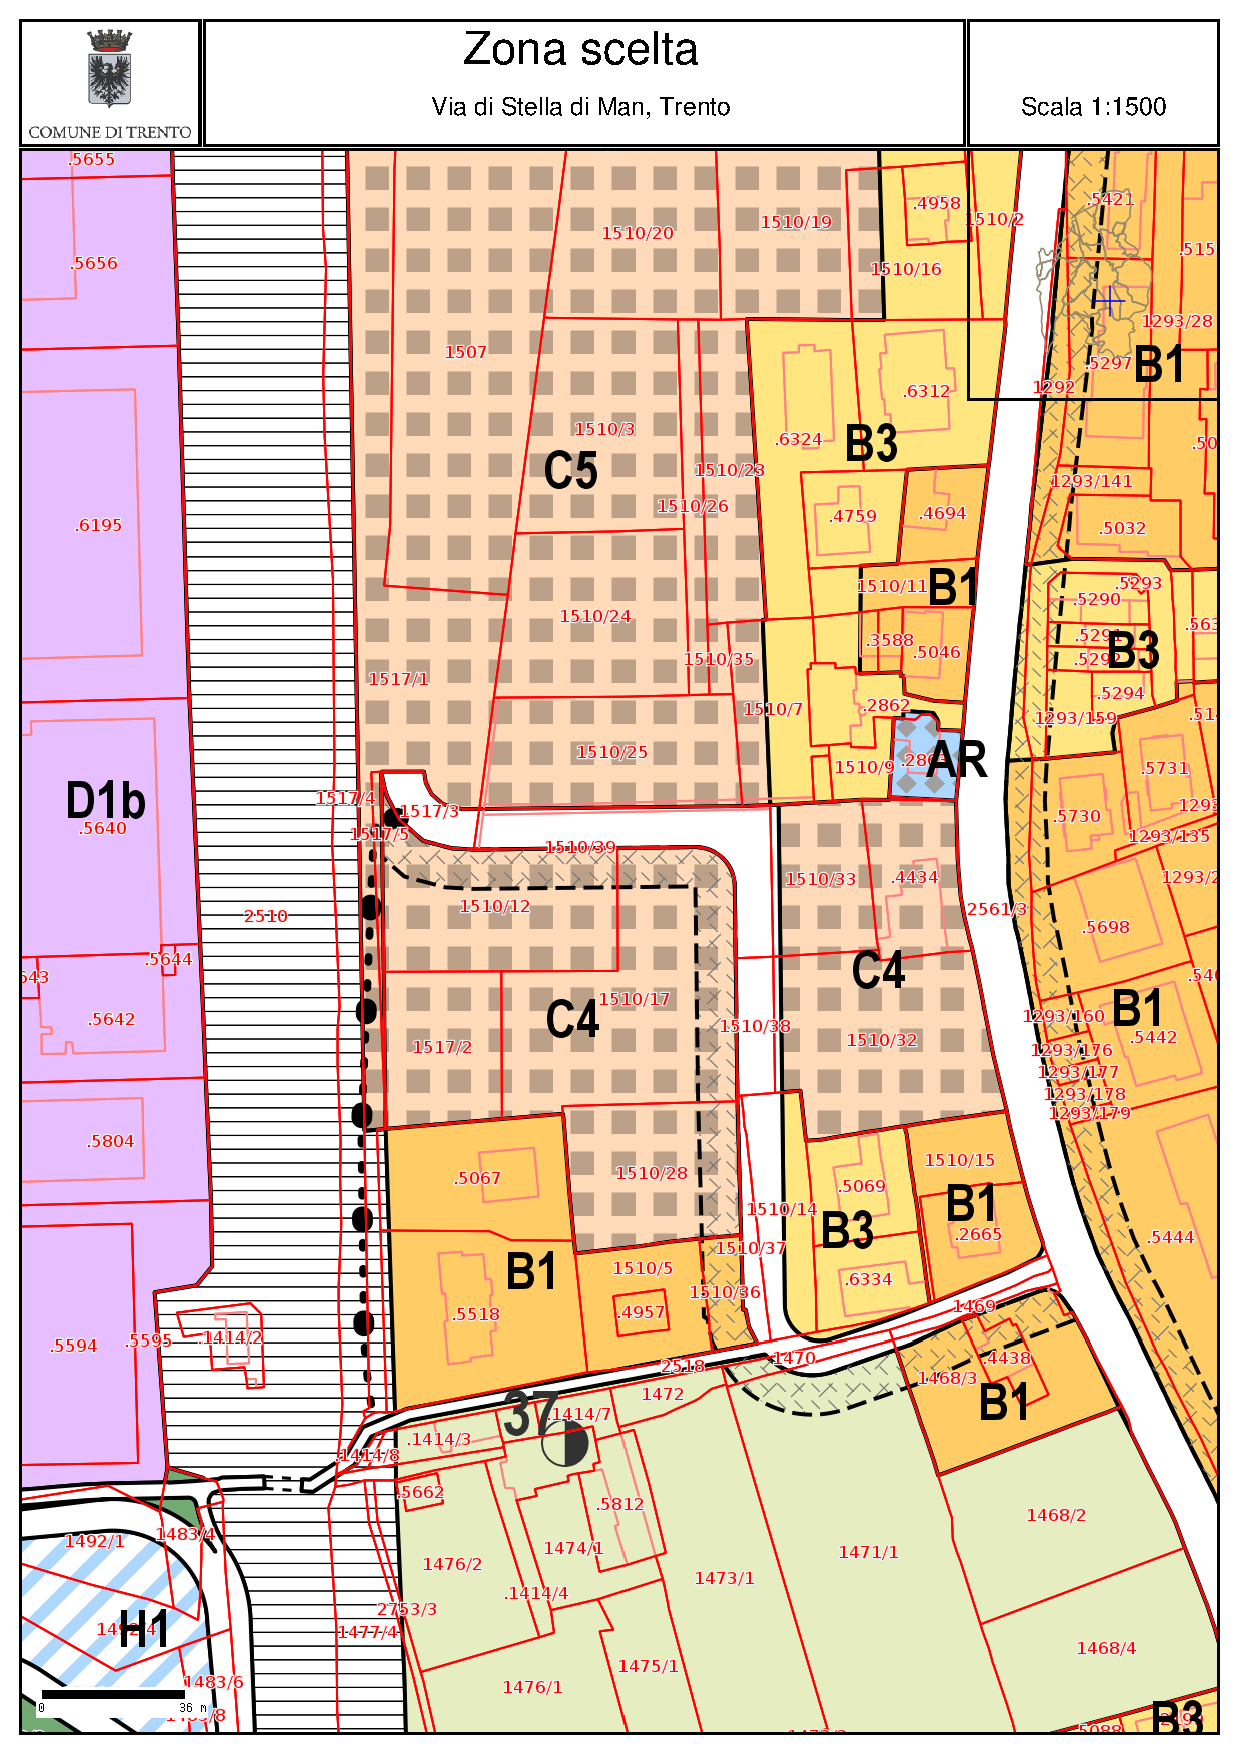
\includepdf[pages={1,2},pagecommand={\thispagestyle{plain}},addtotoc={1,section,2,Zonizzazione dello stato zero,Edificio}]{img/Zonizzazione1.pdf}
\includepdf[pages={1},pagecommand={\thispagestyle{plain}}]{img/Zonizzazione2.pdf}
%WBS:
%\clearpage
%\phantomsection
%\label{WBS}
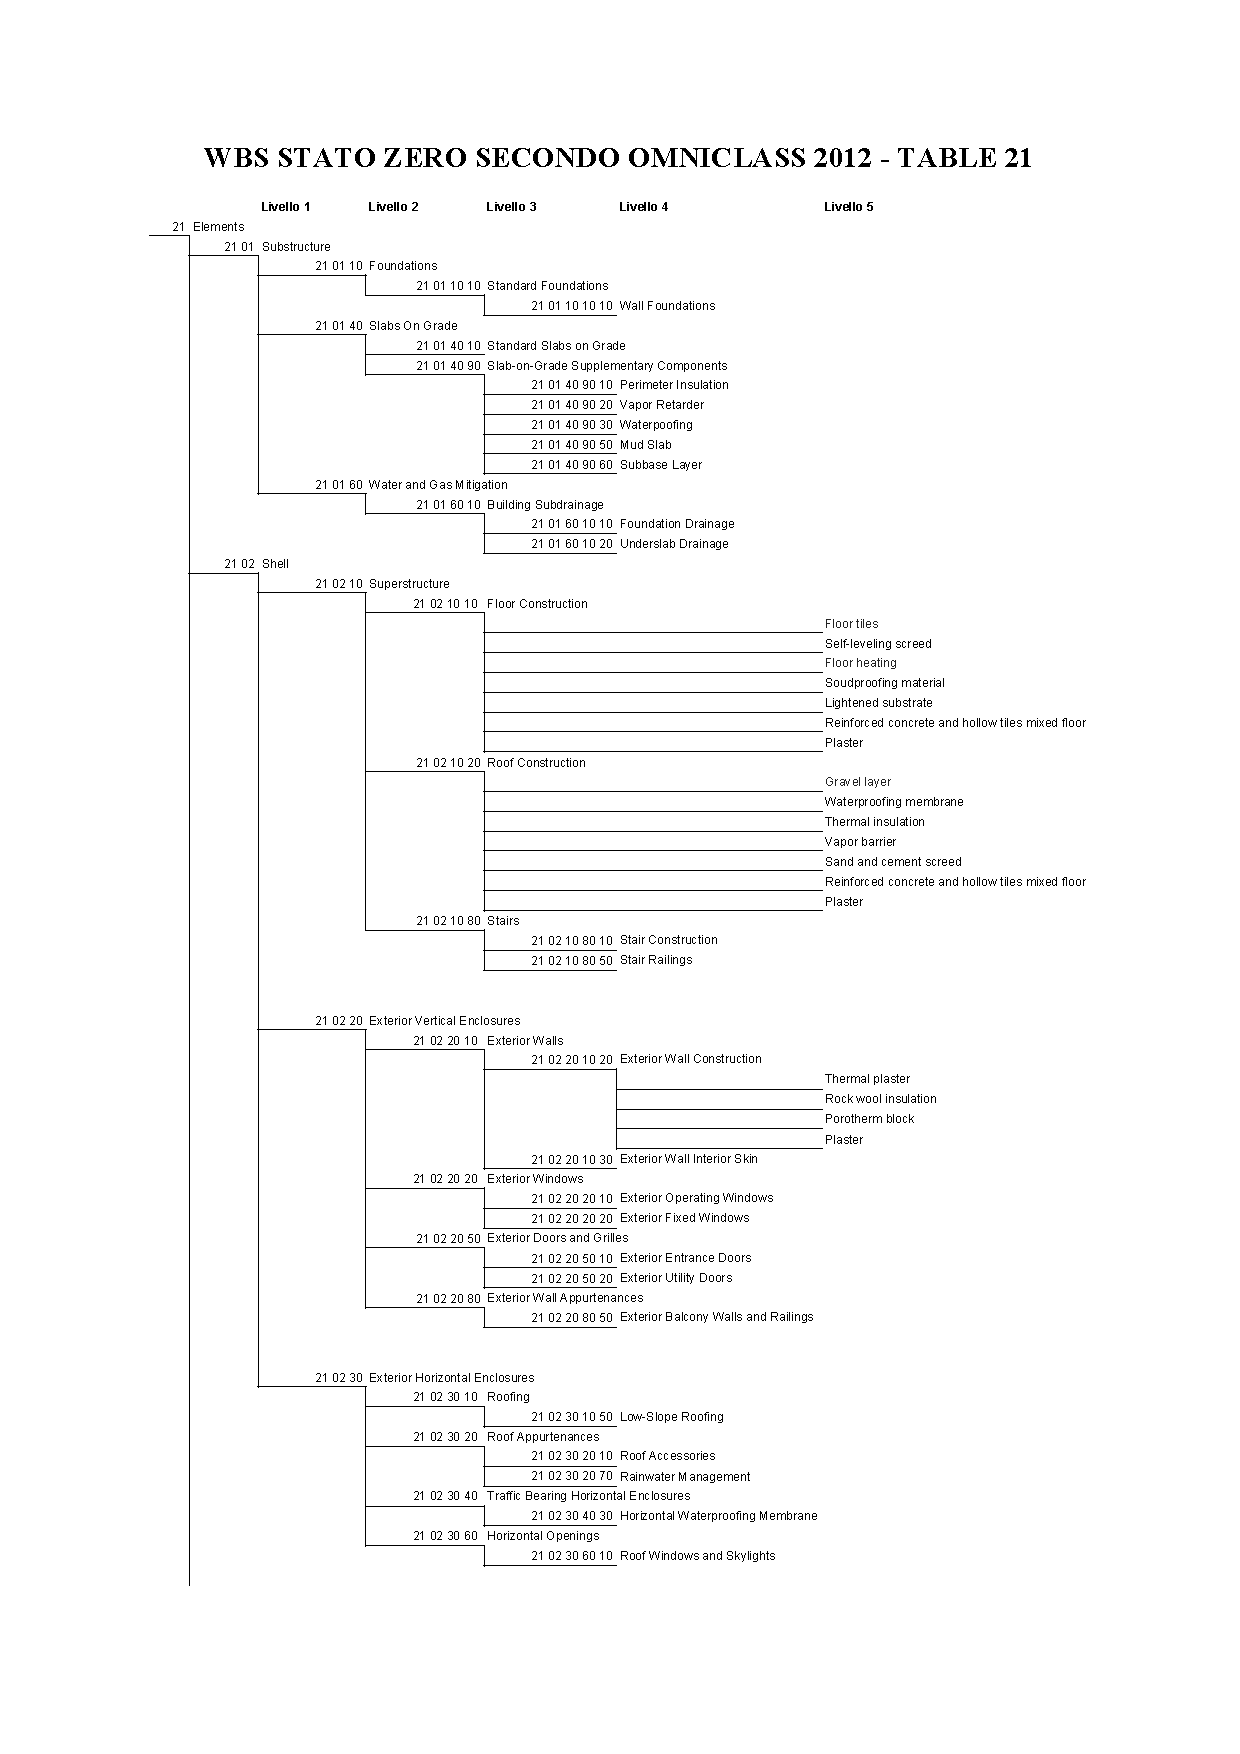
\includepdf[pages={1,2},pagecommand={\thispagestyle{plain}},addtotoc={1,section,2,WBS dello stato zero,WBS}]{img/WBStable21.pdf}
%Conputo strutture perimetrali:
%\clearpage
%\phantomsection
%\label{STRUTcostoMateriale}
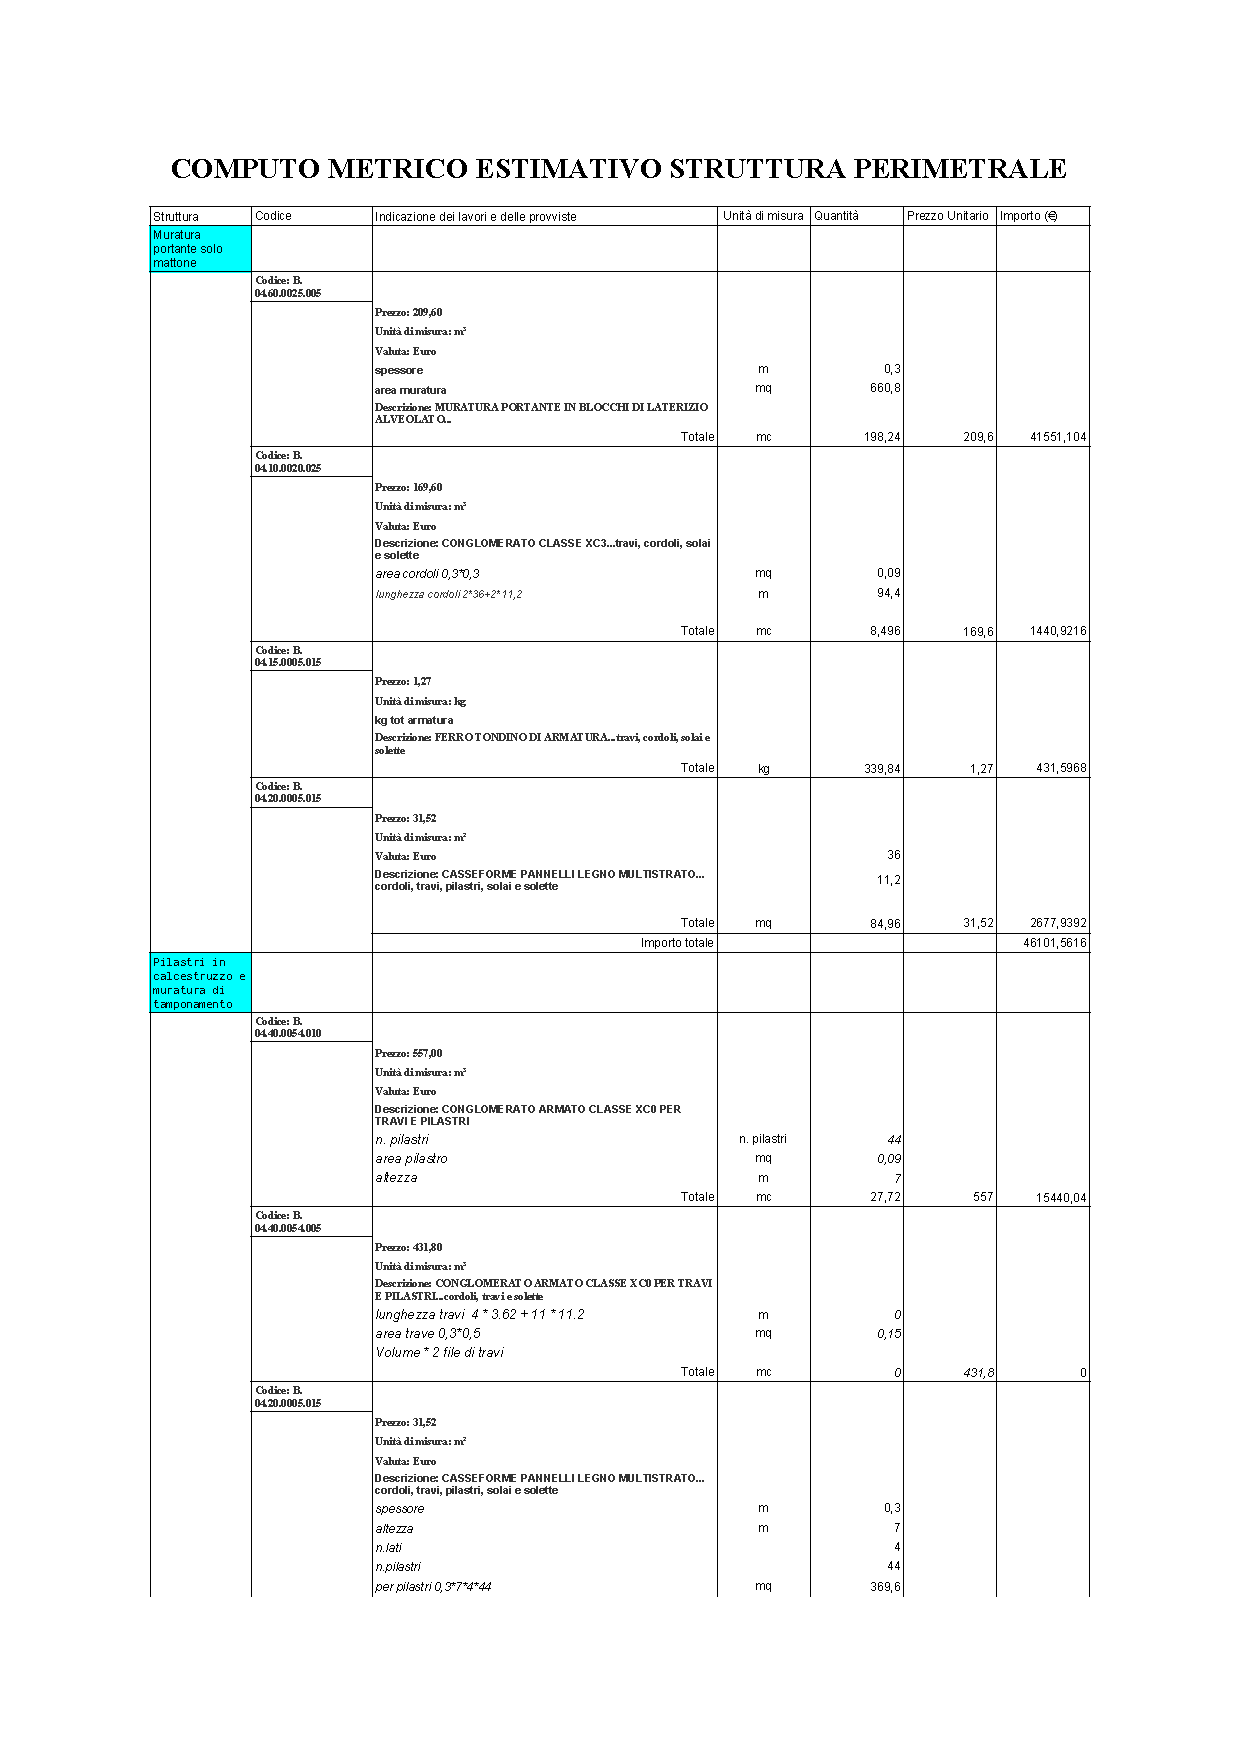
\includepdf[pages={1-3},pagecommand={\thispagestyle{plain}},addtotoc={1,section,2,Computo metrico estimativo struttura perimetrale,STRUTcostoMateriale}]{img/STRUTcostoMateriale.pdf}
%Conputo strutture interne e solai:
%\clearpage
%\phantomsection
%\label{STRUTMuraturaTotaleIntESol}
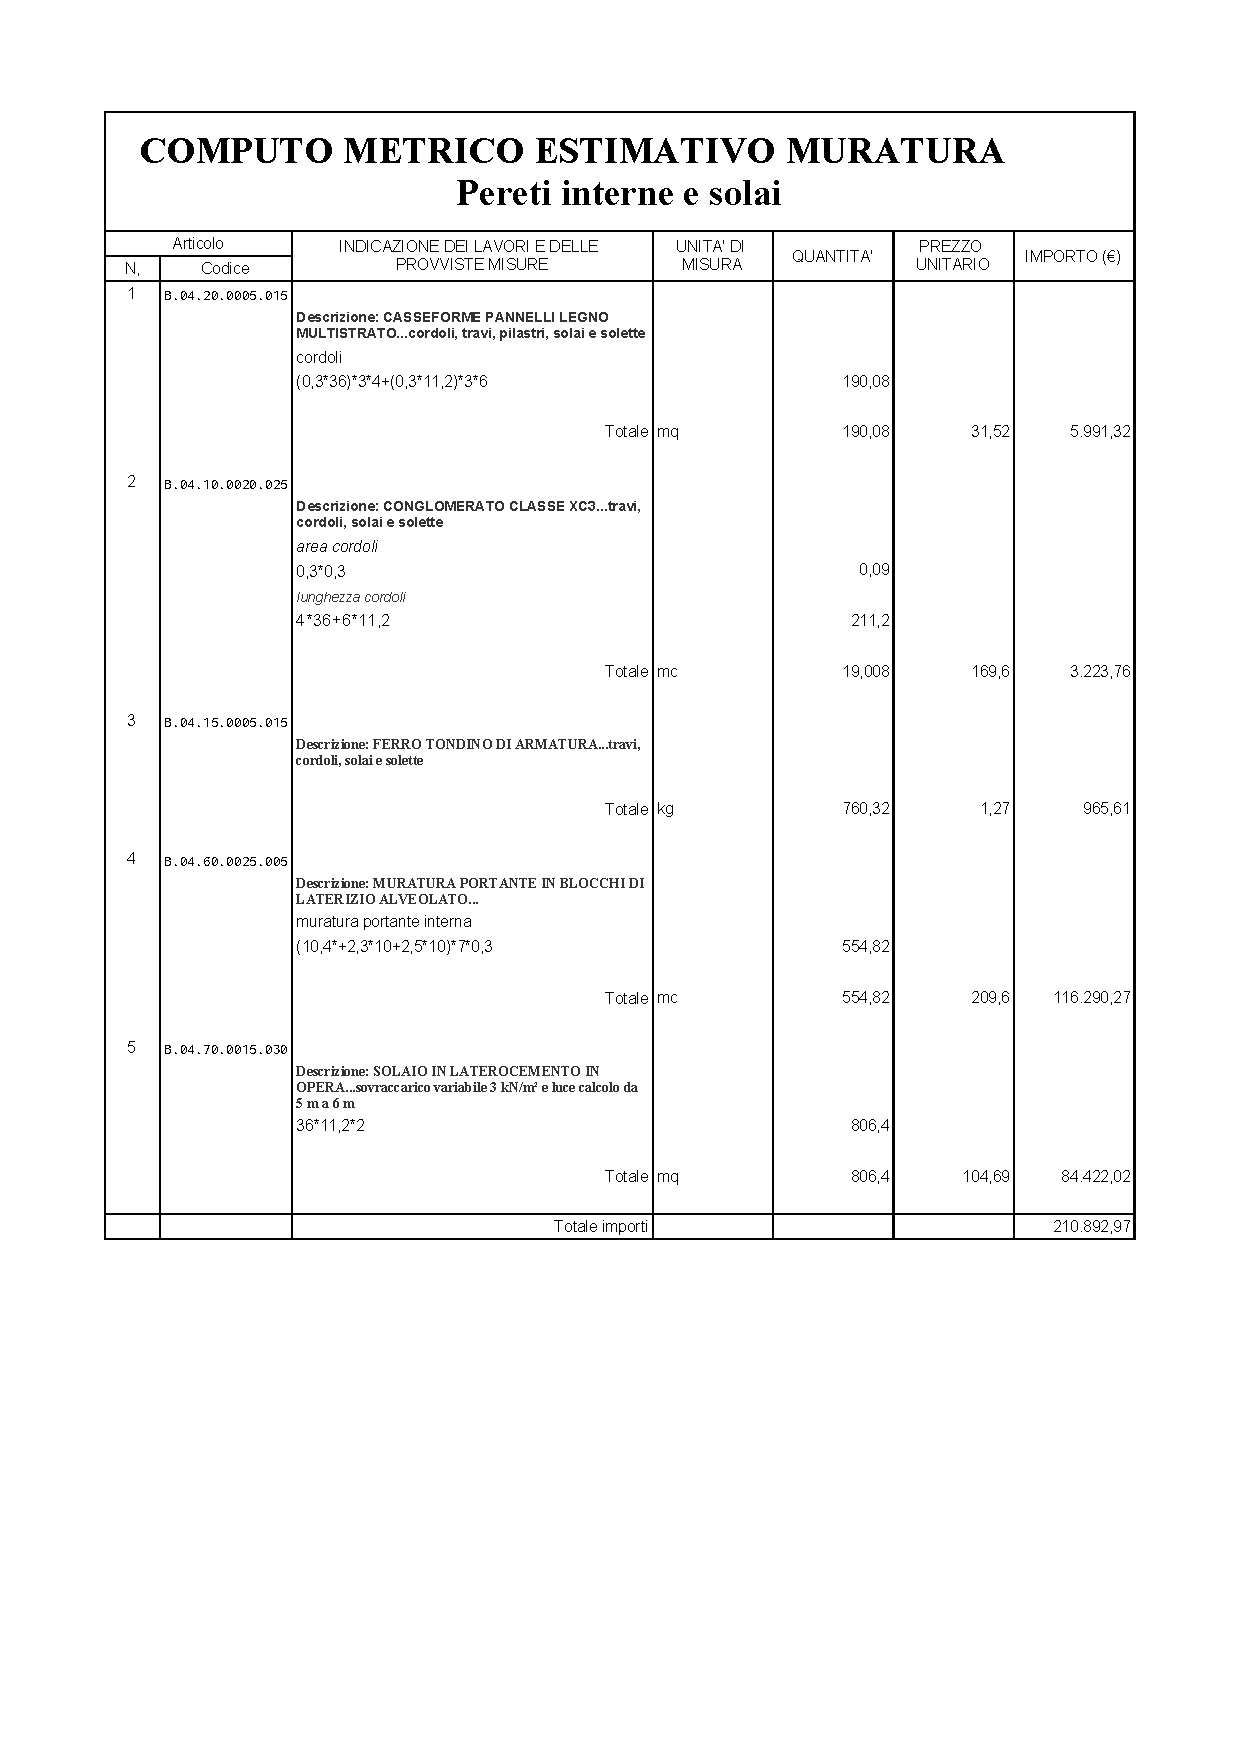
\includepdf[pages={1},pagecommand={\thispagestyle{plain}},addtotoc={1,section,2,Computo metrico estimativo struttura pareti interne e solai intermedi e di copertura,STRUTMuraturaTotaleIntESol}]{img/STRUTMuraturaTotaleIntESol.pdf}
%
\clearpage
\phantomsection
\label{STRUTXLaMTotaleIntESol}
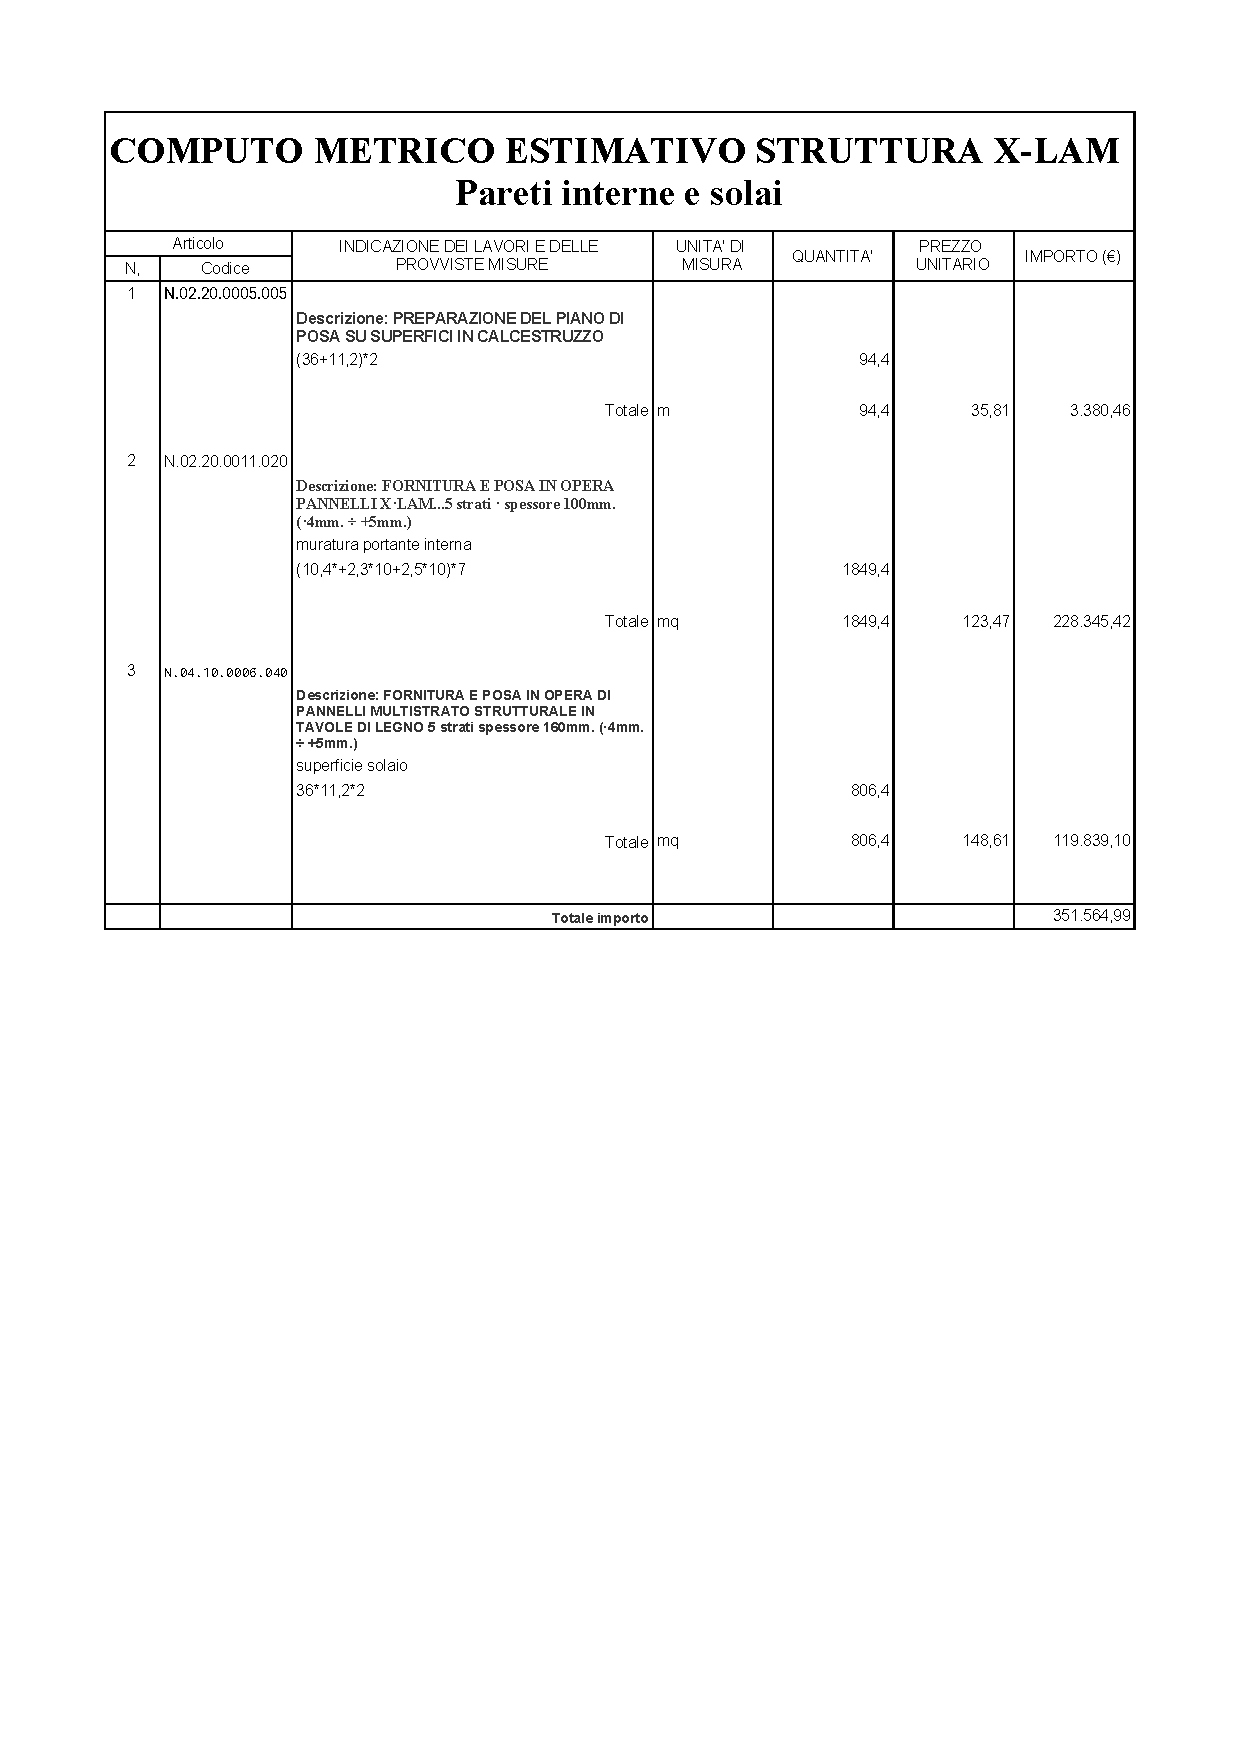
\includepdf[pages={1},pagecommand={\thispagestyle{plain}}]{img/STRUTXLAMTotaleIntESol.pdf}